\section{Extra Search Stalls Learned-Model Planners While Lifting Exact-Simulator Search}\label{sec:pressure}

\begin{figure*}[t]
\centering
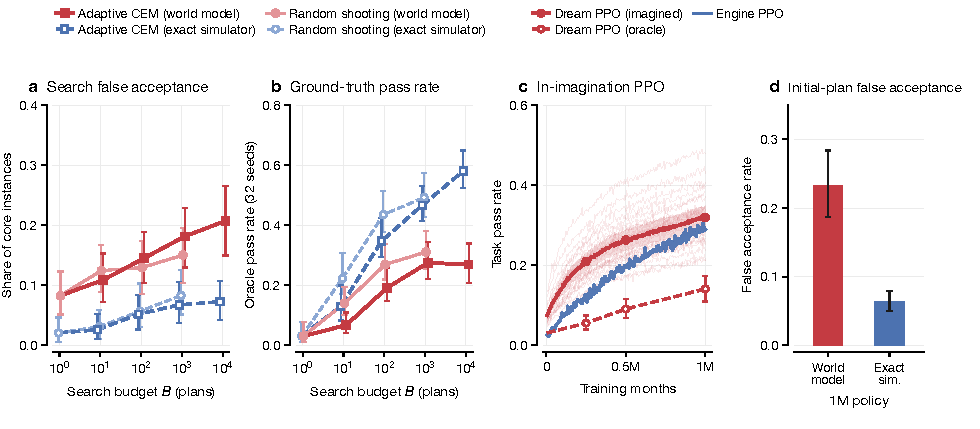
\includegraphics[width=\textwidth]{figures/fig_pressure.pdf}
\caption{\textbf{Escalating optimisation pressure widens ground-truth success shortfall alongside persistent excess false acceptance.} Primary \SizeM{} world model (crimson) paired against the exact-simulator reference on fresh seeds (steel blue). \textbf{a}, False acceptance vs.\ plans scored $B$ for random shooting (circles) and adaptive seeded CEM (squares, anchored at shared unoptimised $B ={}$\Bp{0}) across \PaOnInstances{}. \textbf{b}, Ground-truth pass rate on the \OracleSeeds-seed oracle, opening a \PaTenThouShort{} shortfall at $B ={}$\Bp{4}. \textbf{c}, High-resolution \PrUpdates-step PPO learning trajectories across all \RlCkptsDone{} ladder checkpoints (\RlRunsDone{} runs; imagined pass rate vs.\ \OracleSeeds-seed oracle pass rate and engine-trained PPO). \textbf{d}, After \RlMonths{} imagined months, initial-trajectory verdict false acceptance across the ladder vs.\ the exact-simulator reference (error bars denote \CILevel{} per cent cluster-bootstrap intervals; Tables~\ref{tab:axis} and~\ref{tab:main}).}
\label{fig:pressure}
\end{figure*}

Figure~\ref{fig:pressure} orders four regimes by optimisation pressure. We progress from single unoptimised plans ($B ={}$\Bp{0}) and non-adaptive random shooting (\Bp{3}) to adaptive cross-entropy search (\Bp{4}), in-imagination PPO (\RlMonths{} steps), and monthly closed-loop replanning, before examining sixfold extended one-step training.

\subsection{Unoptimised Calibration and Random Shooting}

On the two-epoch ladder, optimism appears before any search begins. Evaluating a single identical logged plan per start, the primary model falsely accepts \RandOneHack{} \ci{\RandOneHackCI} of core instances versus \RandOnePerfHack{} for the exact-simulator reference, a paired excess of \RandOneDiff{} \ci{\RandOneDiffCI} (Table~\ref{tab:main}). Scaling random shooting to $B ={}$\Bp{3} lifts raw false acceptance under both judges via the optimiser's curse while holding model excess steady at \RandThouDiff{} \ci{\RandThouDiffCI} on the core and \ReplRandThouAllDiff{} \ci{\ReplRandThouAllDiffCI} across all \AllCities{} cities. By contrast, when open-loop rollouts carry uniform upward bias yet preserve trajectory rankings, as in our external TD-MPC2 software check (Appendix~\ref{app:external}), shooting lowers false acceptance from \CheetahRandOneHack{} and \WalkerRandOneHack{} at \Bp{0} to \CheetahRandThouHack{} and \WalkerRandThouHack{} at \Bp{3}.

On Micropolis, higher shooting budgets do not produce a statistically established rise in excess false acceptance. Instead, they widen the ground-truth discovery gap, which grows from zero at \Bp{0} to \RandThouShort{} \ci{\PaRandThouShortCI} at \Bp{3} (\RandThouOrAcc{} vs.\ \RandThouPerfOrAcc{} exact reference; Table~\ref{tab:main}). Conditional on world-model approval at \Bp{3}, the oracle rejects \RandThouCondRej{} \ci{\RandThouCondRejCI} of plans (vs.\ \RandThouPerfCondRej{} reference), while the model falsely rejects \RandThouFalseRej{} of truly passing selections (vs.\ \RandThouPerfFalseRej{}). Roughly half of exploited plans are deep failures rather than near-misses, with \DepthRandLow{} of \DepthRandN{} passing fewer than \DepthCut{} of oracle seeds (median pass share \DepthRandMedian{}; Appendix~\ref{app:axis}). Screening the top choice once on the simulator eliminates false acceptance yet recovers none of the \RandThouShort{} lost ground-truth success.

\subsection{Adaptive Cross-Entropy Search to \Bp{4} Evaluations}

Unlike random shooting over fixed logs, adaptive seeded CEM iteratively mutates elites toward states the world model rewards (Appendix~\ref{app:searches}). Inside the exact simulator, it matches random shooting at \Bp{3} (\AdThouPerfOrAcc{} vs.\ \RandThouPerfOrAcc{}) and climbs further at \Bp{4}. Inside the primary world model at \Bp{3}, false acceptance reaches \AdThouHack{} \ci{\AdThouHackCI} (excess \AdThouDiff{} \ci{\AdThouDiffCI}), while ground-truth pass rate trails at \AdThouOrAcc{} \ci{\AdThouOrAccCI} versus \AdThouPerfOrAcc{} \ci{\AdThouPerfOrAccCI}.

Across \Bp{1} to \Bp{4} (Figure~\ref{fig:pressure}a,b; Table~\ref{tab:axis}), world-model ground-truth pass rates climb roughly fourfold from \PaTenOrAcc{} to \PaThouOrAcc{} at \Bp{3} before stalling at \PaTenThouOrAcc{} at \Bp{4}. Exact-simulator discovery keeps rising from \PaTenPerfOrAcc{} to \PaThouPerfOrAcc{} and \PaTenThouPerfOrAcc{}. Expanding compute tenfold from \Bp{3} to \Bp{4} adds \PaPerfOrAccRise{} real pass rate in the exact simulator (corrected \PaPerfOrAccRiseCorrCI) yet yields \PaEmuOrAccRise{} inside the world model (corrected \PaEmuOrAccRiseCorrCI), absorbing extra search into model-specific optima. Excess false acceptance remains elevated from \PaTenExcess{} to \PaTenThouExcess{} \ci{\PaTenThouExcessCI}. \PressureRiseSentence{} \PaShortSentence{} Relative shortfall stays near half of exact-simulator discovery across all four budgets (Table~\ref{tab:axis}; Appendix~\ref{app:axis}).

\subsection{Out-of-Sample Consistency Across \AllCities{} Held-Out Cities}\label{sec:replication}

Evaluating the primary checkpoint on the disjoint \XCities-city expansion split confirms split consistency (Table~\ref{tab:repl}). At $B ={}$\Bp{3}, random shooting records \ReplRandThouEightyDiff{} \ci{\ReplRandThouEightyDiffCI} excess false acceptance versus \ReplRandThouFortyDiff{} on the \HeldOutFamilies-city core (difference \ReplRandSizeDiff{} \ci{\ReplRandSizeDiffCI}). Adaptive CEM similarly records \ReplAdThouEightyDiff{} \ci{\ReplAdThouEightyDiffCI} versus \AdThouDiff{} (difference \ReplAdSizeDiff{} \ci{\ReplAdSizeDiffCI}). Pooled across all \AllCities{} cities (\AllInstances{} instances), random-shooting excess stays steady from \ReplRandOneAllDiff{} at \Bp{0} to \ReplRandThouAllDiff{} \ci{\ReplRandThouAllDiffCI} at \Bp{3} (paired shift \ReplRandRiseAll{} \ci{\ReplRandRiseAllCI}), again showing persistent excess rather than an established budget slope.

\subsection{In-Imagination Reinforcement Learning}

Training closed-loop PPO policies \citep{schulman2017ppo} for \RlMonths{} imagined steps across all \RlCkptsDone{} checkpoints (\RlRunsDone{} runs; Appendix~\ref{app:rl}) reveals parallel policy-level exploitation (Figure~\ref{fig:pressure}c,d). Under our \KVerdict-rollout verdict rule, initial policy trajectories incur \RlAxExcess{} \ci{\RlAxExcessCI} excess false acceptance across the ladder (\RlAxHack{} vs.\ \RlAxPerfHack{} exact reference) and \RlMainAxExcess{} \ci{\RlMainAxExcessCI} on the primary model.

PPO policies succeed in \RlDream{} \ci{\RlDreamCI} of imagined episodes yet pass the \OracleSeeds-seed oracle on only \RlOracle{} \ci{\RlOracleCI}, an optimism gap of \RlGap{} \ci{\RlGapCI} (Table~\ref{tab:rlfam}). Identical PPO policies trained directly on the C++ engine (\RlEngSeeds{} seeds per family) incur a \RlEngGap{} stochasticity gap. Subtracting this baseline yields a net optimism excess of \RlGapExcess{} \ci{\RlGapExcessCI}, rising from \RlQtrGap{} at quarter budget to \RlGap{} at \RlMonths{} steps. Executed closed loop on the engine, world-model policies pass \RlClosed{} \ci{\RlClosedCI}, trailing engine-trained PPO by \RlLostClosed{} \ci{\RlLostClosedCI} closed loop and \RlLostFull{} \ci{\RlLostFullCI} open loop. Continuous margin inflation averages \RlInfl{} behaviour-mix standard deviations. \RlInflIntervalSentence{}

\ReplanParagraph

\ifRpOn\ifRpKeptEmuOn Abandoning an in-progress spatial build plan without switching hysteresis causes destructive plan thrashing even inside the exact simulator (Appendix~\ref{app:ablations}). The \RpSwitchSe{}-standard-error gate retains the incumbent plan in \RpKeptEmuMin{}--\RpKeptEmuMax{} (world model) and \RpKeptPerfMin{}--\RpKeptPerfMax{} (exact simulator) of \RpKeptOf{} replanning months, characterising conservative plan commitment with occasional revision rather than step-by-step MPC.\fi{} On this \RpN{}-instance subset, open-loop realised false acceptance is slightly lower under the world model than in the exact simulator (\RpEmuOpenHack{} vs.\ \RpPerfOpenHack{}), explaining why closed-loop excess of \RpRaEst{} represents a \RpRbEst{} shift over open loop.\fi

\subsection{Longer One-Step Training Flips Optimism to Pessimistic Collapse}\label{sec:extended}

To test whether two-epoch rollout drift and false acceptance stem simply from early stopping, we trained a single seed of the primary \SizeM{} full-data architecture sixfold longer (\ExtTrSamples{} examples, \ExtTrEpochs{} epochs; Table~\ref{tab:extended}, Appendix~\ref{app:extended}). Held-out variational ELBO rises monotonically by \ExtTrTestElboGain{} nats, one-month F1 edges up to \ExtTrTestFOne{}, and \RollA-month funds error falls from \TestMainFunds{} to \ExtTrTestFunds{}. Yet \Horizon-month spatial drift worsens even on training cities. Mean spatial-overlay copy ratio climbs from \ExtTrBaseMeanOv{} to \ExtTrMeanOv{} (\ExtTrGeCopy{} of \HorOverlays{} above copy) and open-loop powered-zone error rises from \HorPowEmu{} to \ExtTrPowMae{} tiles alongside growing latent KL (\ExtTrKlStart{} to \ExtTrKlEnd{} nats), consistent with compounding teacher-forced conditionals or prior-posterior mismatch.

Under search and RL, this spatial drift flips miscalibration from optimistic false acceptance to pessimistic rejection rather than curing it. Across milestones on all \AllCities{} cities, single-plan excess stays positive through \ExtTrMileEightEpochs{} epochs before crossing zero at \ExtTrMileTenEpochs{}--\ExtTrEpochs{} epochs as false rejection climbs to \ExtTrRandOneAllFalseRej{} (Table~\ref{tab:extended}). At \Bp{4} adaptive CEM, raw false acceptance drops to \ExtTrTenThouHack{} \ci{\ExtTrTenThouHackCI} by driving false rejection from \ExtTrMainTenThouFalseRej{} to \ExtTrTenThouFalseRej{} \ci{\ExtTrTenThouFalseRejCI} and collapsing model self-acceptance to zero on \ExtTrZeroAccFams{} of five task families (\emph{grow}, \emph{solvent}, and \emph{recover}). Pooled ground-truth pass rates still stall between \Bp{3} and \Bp{4}, leaving a \ExtTrTenThouShort{} \ci{\ExtTrTenThouShortCI} shortfall. Under PPO (\ExtTrRlRuns{} runs), better scalar accounting lifts \emph{treasury} oracle pass rate by \ExtTrRlTreasOracleDiff{} \ci{\ExtTrRlTreasOracleDiffCI}, though its initial-plan verdict excess remains \ExtTrRlTreasAxExcess{} \ci{\ExtTrRlTreasAxExcessCI}. Collapsed spatial rollouts meanwhile cut closed-loop pass rates across the four spatial families from \ExtTrMainRlSpatClosed{} to \ExtTrRlSpatClosed{} (difference \ExtTrRlSpatClosedDiff{} \ci{\ExtTrRlSpatClosedDiffCI}). We retain the two-epoch checkpoint as primary because it avoids zero-acceptance collapse and achieves higher pooled PPO real success.
